\section{Description And Methodology}


\subsection{Initial Setup}
In this assignment the following peripherals need to be configured, buttons, LEDs, DAC, and some timer. The buttons are needed to allow interaction with the board. The buttons are configured to play different sounds when pushed. 




\subsection{Sound Wave Synthesis}
Sound is realised through sound waves which is created by oscillations. "An oscillator generates a consistent, repeating signals". These consistent signals can be used to create waves at various frequencies. Sound is actually the properties of the waves generated, with respect to frequency, amplitude, and period. The frequency determines the tone of the sound, the amplitude the strength, and the period the duration of the sound.  

There are various different approaches for generating these sound waves. The different waves have slightly different properties in regard to sound. To name a few different waves we have the sine wave, sawtooth wave, triangle wave and the square wave. These waves produces different sound characteristics {\bf more on this ? Sources and shit like that}. 

In case of this assignment, we have crated two different kind of waves, the square wave and the sawtooth wave. The square wave is created by calculating discrete samples based on the tone frequency and the oscillator frequency. Oscillator frequency divided by the tone frequency decides how often the values to the DAC should alternate, thereby producing an approximation of the note. The different notes supported by the program is as follows, A, B, C, D, E, F, and H.


\begin{figure}[H]
  \centering
  % Trim er [left bottom right top]
  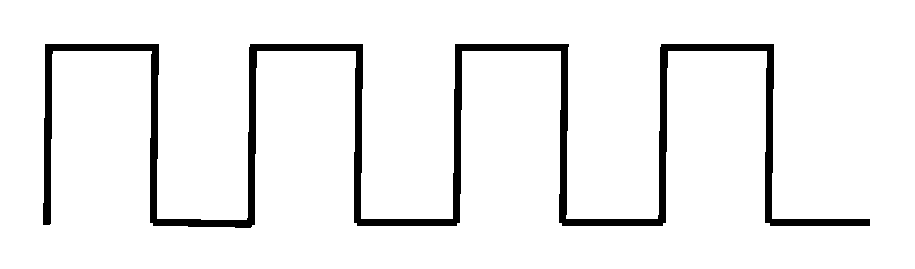
\includegraphics[clip, trim=0cm 0cm 0cm 0cm, width=4cm]{fig/square_wave.pdf}
  \caption{Square wave}
\end{figure}

\begin{figure}[H]
  \centering
  % Trim er [left bottom right top]
  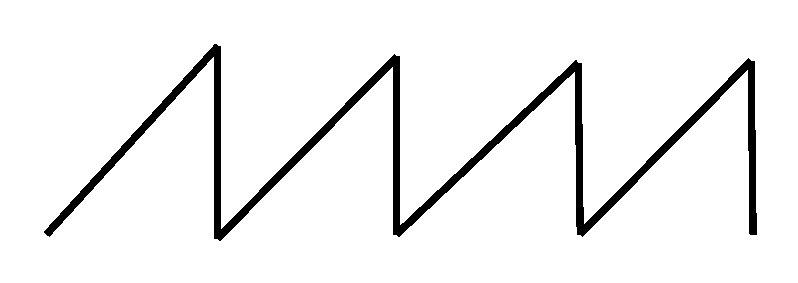
\includegraphics[clip, trim=0cm 0cm 0cm 0cm, width=4cm]{fig/sawtooth.pdf}
  \caption{Sawtooth wave}
\end{figure}



\subsection{Sound Sampling}
Sound can also be generated through pre computed samples. With this approach the sound waves are generated on some other platform. The samples produced are approximations to already existing sound waves. 


\subsection{Energy Optimization}
The EFM32GG microcontroller has a rich set of features regarding improving energy efficiency, where the main focus is turning of components that are not in use, or tuning their performance. We have utilised many of these techniques to improve the power consumption of the program, where our main goal has been to try to exploit the various energy levels that the microcontroller has to offer, preferably being able to achieve EM3 and turn of every component not in use. 

Various techniques were employed to reach this goal. As it turned out, achieving deep sleep and sleep on exit proved to be more complicated than first imagined. During deep sleep mode the high frequency oscillator was turned off. This oscillator was used to clock both the DAC and the timer. When entering EM3 this produced some unexpected bugs. On entering EM2 the program started to behave non-deterministic. As it turned out, both the DAC and the timer was clocked by the high frequency oscillator. This directly affected the interrupts produced by the timer. This problem was solved by introducing the low energy timer. This timer is able to run as low as EM2 and EM3 depending on the oscillator used. For producing sound, the 32.768 KHz oscillator was used. This timer replaced the old timer, and only caused some minor changes to made in the already existing code. In particular, the frequency used to generated was changed to accommodate the new oscillator frequency. Instead of  using a sample rate of 48000, the new oscillator was able to produce 32768 interrupts every second. This implied a maximum sample rate of 32768. Fortunately, our tone frequencies were sufficiently low to accommodate this change in sample frequency. However, while this reduced the energy consumption, there were still some problems with the DAC, as entering a lower energy mode caused the DAC to continue producing static sound. As it turns out, configuring the DAC with continuous mode will not be able to maintain the voltage levels when entering deep sleep. This caused the voltage levels to fluctuate, and create a static background sound. Fortunately, the DAC also support another mode, sample/hold mode. During sample/hold mode, the DAC core converts on a triggered conversion and then holds the output in a sample/hold element. When not converting, the DAC is turned of between samples, which reduces the power consumption. The sample/hold element will hold the element for a certain time without needing a refresh conversion\cite{EFM32GG-rm}. Switching to this mode not only fixed our bug, but also further decreased the energy consumption. This change from continuous mode to sample/hold mode is achieved by changing the value written to the $DAC0\_CTRL$ register from 0x50010 to 0x50014. 

These techniques allow the code to enter deep sleep mode, and also allow utilisation of sleep on exit. This is was accomplished by writing the value 6 to the SCR register setting the deep sleep and deep sleep on exit bit. Entering EM3 is then achieved by calling the WFI instruction.

These techniques combined proved to be very beneficial regarding the energy efficiency. However, even further improvements could be made. While the high frequency oscillator was turned off during deep sleep, the energy timer would still consume power. To allow the program achieve even better decrease in power consumption, we implemented functions that could enable/disable these components. Said components were only enabled when needed, and disabled during idle mode.




\subsection{User Control}

In order to let a user be able to interact with our setup, the buttons on the gamepad were configured so that different sounds would play when one of them were pressed. Each button was configured to play one specified sound or melody. This was done by reading the value of the $GPIO\_PC\_DIN$ register, and writing this value to a function $play\_melodies(int)$ that would take the $GPIO\_PC\_DIN$ value as an input parameter and play the corresponding melody. One of the challenges in this was to get the DAC to output the entire melody, and not just for the duration in which a button was pressed. To solve this, a pointer variable was used to point to the correct sample array and let the timer run for the entire length of the array in order to play the whole melody. An alternative approach was to declare a global variable and set it to the value of the $GPIO\_PC\_DIN$ register in each of the GPIO-handlers, and use a switch-statement in the low-energy timer function to play the corresponding melody, but the former approach was prefered due to its energy efficiency advantages.

Our setup was as follows:

\begin{table}[ht]
\caption{Buttons and corresponding melodies}
% title of Table
\centering
% used for centering table
\begin{tabular}{c c}
% centered columns (4 columns)
\hline
\hline %inserts double horizontal lines
Button & Melody \\ [0.5ex]
% inserts table
%heading
\hline
SW1 & Mario \\
SW2 & Shoot \\
SW3 & Hit dealt \\
SW4 & Hit received \\
SW5 & Battlefield intro \\
SW6-SW8 & Simple *beep*-noises \\
% [1ex] adds vertical space
\hline
%inserts single line%
\end{tabular}
\label{table:nonlin}
% is used to refer this table in the text
\end{table}











